\documentclass[tikz,border=4pt]{standalone}
\usetikzlibrary{arrows.meta,calc,positioning}
\begin{document}
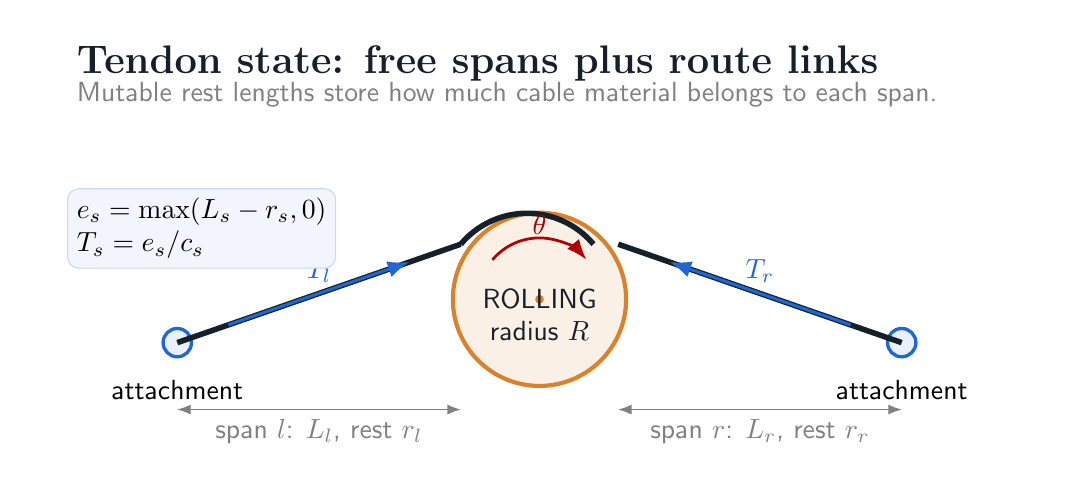
\begin{tikzpicture}[>=Latex, font=\sffamily]
  \definecolor{ink}{HTML}{16202A}
  \definecolor{blue}{HTML}{1F67D2}
  \definecolor{orange}{HTML}{D9822B}
  \draw[fill=white, draw=none] (-0.5,-1.2) rectangle (12.4,4.0);
  \node[anchor=west, font=\bfseries\Large, text=ink] at (0,3.55) {Tendon state: free spans plus route links};
  \node[anchor=west, text=gray] at (0,3.15) {Mutable rest lengths store how much cable material belongs to each span.};

  \coordinate (L) at (1.4,0);
  \coordinate (P) at (6.0,0.55);
  \coordinate (R) at (10.6,0);
  \coordinate (A) at (5.0,1.25);
  \coordinate (B) at (7.0,1.25);

  \draw[fill=blue!10, draw=blue, line width=1.2pt] (L) circle (0.18);
  \draw[fill=blue!10, draw=blue, line width=1.2pt] (R) circle (0.18);
  \node[below=0.35cm of L] {attachment};
  \node[below=0.35cm of R] {attachment};

  \draw[fill=orange!12, draw=orange, line width=1.5pt] (P) circle (1.1);
  \fill[orange] (P) circle (0.055);
  \node[text=ink] at (P) {ROLLING};
  \node[text=ink, below=0.15cm of P] {radius $R$};

  \draw[line width=2pt, color=ink] (L) -- (A);
  \draw[line width=2pt, color=ink] (B) -- (R);
  \draw[line width=2pt, color=ink] (A) arc[start angle=140,end angle=40,radius=1.1];

  \draw[->, blue, line width=1.1pt] ($(L)!0.18!(A)$) -- ($(L)!0.82!(A)$) node[midway, above] {$T_l$};
  \draw[->, blue, line width=1.1pt] ($(R)!0.18!(B)$) -- ($(R)!0.82!(B)$) node[midway, above] {$T_r$};
  \draw[<->, gray] (L |- 0,-0.85) -- (A |- 0,-0.85) node[midway, below] {span $l$: $L_l$, rest $r_l$};
  \draw[<->, gray] (B |- 0,-0.85) -- (R |- 0,-0.85) node[midway, below] {span $r$: $L_r$, rest $r_r$};
  \draw[->, red!70!black, line width=1pt] ($(P)+(140:0.78)$) arc[start angle=140,end angle=40,radius=0.78];
  \node[red!70!black] at ($(P)+(90:0.95)$) {$\theta$};

  \node[draw=blue!25, fill=blue!6, rounded corners, anchor=west, align=left, font=\ttfamily] at (0,1.45)
    {$e_s=\max(L_s-r_s,0)$\\$T_s=e_s/c_s$};
\end{tikzpicture}
\end{document}
